\documentclass{proc}
\usepackage[utf8]{inputenc}
\usepackage{cmap}					% поиск в PDF
\usepackage[T2A]{fontenc}			% кодировка
\usepackage[utf8]{inputenc}			% кодировка исходного текста
\usepackage[english,russian]{babel}	% локализация и переносы
\usepackage{amsmath}
\usepackage{graphicx}
\graphicspath{ {images/} }
\begin{document}

\noindent {\Large \bf Вопросы на ''до свидания''}
\begin{enumerate}
\item \underline{Полнота, точность}

Полнота, она же Recall - сколько фрода мы поймали.

Точность, Precision - сколько не-фрода мы пропустили.

$$Recall = \frac{tp}{tp+fn}$$

$$Precision = \frac{tp}{tp+fp}$$

\item \underline{ROC кривая. Коэфициент Джини.  AUC}

ROC кривая - зависимость true positive от false positive для разных порогов решающего правила.

Коэффициент Джини - максимальное отклонение ROC кривой от диагонали $tp = fp$.

Если система адекватная (не контрпродуктивная), то кривая всегда будет выше диагонали.

AUC - ''area under curve'' - площадь под кривой ROC. Чем выше, тем лучше.

\item \underline{tp, fp, tn, fn}

\begin{center}
    \begin{tabular}{| c | c | c |}
    \hline
    ... & Фрод & Не фрод \\ \hline
    Думаем, что фрод & tp & fp \\ \hline
    Думаем, что не фрод & fn & tn \\ \hline
    \end{tabular}

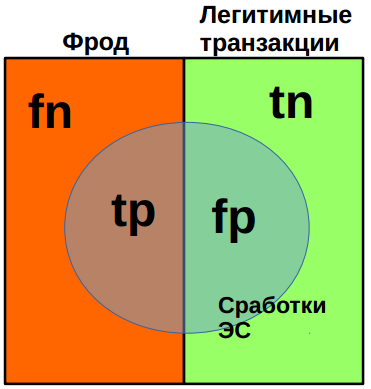
\includegraphics[width=3cm]{tptnfpfn}
\end{center}


\item \underline{классификация}

Есть несколько категорий (напр. фрод$\backslash$не фрод). Необходимо объекты расфасовать по категориям. В ''обучающей выборке'' заранее известно, в какую категорию какой объект входит. 

\item \underline{кластеризация}

Категории заранее неизвестны. Необходимо разбить объекты на несколько ''каких-то'' категорий.

\item \underline{регрессия}

Зная значение функции на каком-то наборе точек, наиболее хорошо приблизить функцию.

\item \underline{идентификация}

Определить, к какой из большого числа категорий принадлежит объект.

\item \underline{обучение с учителем и обучение без учителя}

Supervised$\backslash$Unsupervised learning. При обучении с учителем системе дается какая-то обучающая выборка, для которой задача уже решена (например, при задаче классификации). Без учителя обучающей выборки нет, система сама должна искать закономерности (кластеризация).

\item \underline{признак}

Строго заданная характеристика объекта (например, сумма транзакции в рублях).

\item \underline{класс}

Одна из категорий, принадлежность к которой необходимо определить при решении задачи классификации.

\item \underline{событие, действие, решение}

???

\item \underline{обратная связь}

В общем случае: влияние выхода системы на ее дальнейший вход.

\item \underline{DENY, REVIEW, ALLOW решения ФМ системы RSA}

DENY - заблокировать транзакцию и профиль клиента.

REVIEW - потребовать подтверждение в КЦ.

ALLOW - разрешить без вопросов.

\item \underline{примеры применения машинного обучения для задач информационной безопасности}

Имея транзакции банка, определить фрод.

Предсказать нагрузки на сайт в разное время, дабы не допустить DoS.


\item \underline{экспертная система}

???

\item \underline{выброс}

Нестандартные данные, которые могут помешать классификации.

\item \underline{аномалия}

???

\item \underline{выборка}

Конечный набор объектов, взятый из множества всех возможных объектов.

\item \underline{разделяющая гиперповерхность}

Гиперплоскость в пространстве всех возможных объектов, которая разделяет объекты на классы.

\item \underline{функция штрафа}

Некая функция, символизирующая, насколько ''плохо'' был классифицирован объект. Обычно функция расстояния или просто +1 за каждую точку не в своем классе. Задача классификации сводится к задаче минимизации функции штрафа.

\item \underline{логистическая функция}

$$f(\pm d(x_1,x_2))=f(d)=\frac{1}{1-e^{-\alpha \times d}}$$

Используется в качестве функции штрафа.

\item \underline{ансамбль}

Мнения нескольких систем так или иначе аггрегируются в одно (например, функцией голосования).

\item \underline{дерево решений}

Дерево, в каждом узле которого находится условие, определяющее, к какому из детей надо перейти. В листьях содержатся классы. Каждый объект спускается по дереву в соответствии с условиями, пока не попадет в класс.

\item \underline{бутстрепинг}

Генерация выборки размера $N$ из подвыборки размера $n \ll N$ путем выбора с повторением.

\item \underline{бутстреп аггрегация}

Она же bagging. Тот же ансамбль на классификаторах.

Обобщение одного и того же классификатора на различных подвыборках или случайных параметрах, которые различны при каждой новой подгонки.

\item \underline{подгонка (fitting)}

Настройка параметров классификатора с помощью обучающих выборок.

\item \underline{проверка (scoring)}

Оценка качества классификатора на тестовой выборке.

\item \underline{переобучение (overfitting)}

Явление, когда модель слишком точно подогнана под обучающие данные, видя закономерности в случайном шуме. Такая модель может работать хуже на больших данных.

\item \underline{пакеты pandas, numpy, scikit-learn, matplotlib}

Библиотеки для Python.

Pandas - структуры данных.

numpy - матрицы, математика.

scikit-learn - машинное обучение

matplotlib - графики
\end{enumerate}

\end{document}
